\chapter{Experimental Results}
\label{chap:Results} 

\section{Reconstruction}

\subsection{Quantitative Results}

\subsubsection{GMM}

All proposed methods are able to increase the main network's accuracy and validation accuracy.
Also, the accuracy of the verification network is increased.
It is interesting to note that even though nearly all methods decrease the 
the cross-entropy, the l2-error of the distortion always increases
- for a larger number of samples, the data set cross-entropy is reported as infinity.
This is due to floating point precision errors that arise even with overflow measures in place.
However, it is important to remember that the loss function used in the optimization process
is a composite loss from the proposed loss between the statistics
and the original cross-entropy loss used in the optimization of the neural network.
\[
    r_{stats} \loss(\set A, \set B) + r_{crit}\loss_{crit}(\set B, y_{\set B})
\]
Since, by itself, the original criterion loss alone already performs quite well, 
it can be said that the proposed losses act as a kind of regularization 
by incorporating more knowledge about the target data distribution that prevent overfitting
of the source data set.
A comparison of the results for the case $r_{crit}=0$ can be found in \cref{tab:gmm_results_raw}

The results shown in \cref{tab:gmm_results_raw} confirm the assumption that,
without any class information, no method is able to achieve good results.

In this scenario, two methods, namely NN CC and RP CC seem to give 
better generalization scores 
(validation and verification accuracy) than when the original cross-entropy loss 
$\loss_\text{crit}$ is included.
But it is hard to explain the lower cross-entropy when leaving out 
$\loss_\text{crit}$, which is specifically designed to minimize the cross-entropy.
Nevertheless, it is important to note that scores can fluctuate a fair amount and more 
experiment runs are necessary to give a clearer picture.

\begin{table}[!htbp]
\centering
\footnotesize
\pgfplotstabletypeset[
results,
gmm,
display columns/0/.style={column name=\textbf{Baseline}, column type=l, string type},
]{figures/reconstruction_GMM_baseline.csv}
\caption{GMM baseline scores}
\label{tab:gmm_baseline}
\end{table}

\begin{table}[!htbp]
\centering
\footnotesize
\pgfplotstabletypeset[
results,
gmm,
every row 6 column 1/.style={highlight},
every row 8 column 1/.style={highlight},
every row 10 column 1/.style={highlight},
every row 11 column 1/.style={highlight},
every row 7 column 2/.style={highlight},
every row 4 column 3/.style={highlight},
every row 8 column 4/.style={highlight},
every row 8 column 5/.style={highlight},
]{figures/reconstruction_GMM_results.csv}
\caption{Metrics on reconstruction results after 100 optimization epochs on GMM data set}
\label{tab:gmm_results}
\end{table}

\begin{table}[!htbp]
\centering
\footnotesize
\pgfplotstabletypeset[
results,
gmm,
every row 1 column 1/.style={highlight},
every row 7 column 2/.style={highlight},
every row 7 column 3/.style={highlight},
every row 4 column 4/.style={highlight},
every row 7 column 5/.style={highlight},
]{figures/reconstruction_GMM_results_raw.csv}
\caption{Metrics on reconstruction results after 100 optimization epochs for $r_\text{crit}=0$ on GMM data set}
\label{tab:gmm_results_raw}
\end{table}


When reviewing the trajectories of the scores, many of the methods show that soon after
 the loss passes a reference value - the same loss calculated on a batch of 
unperturbed data - the l2-error is seen to increase. This can be seen in \cref{fig:metrics_GMM_l2_increase}.

\begin{figure}[!htbp]
    \centering
    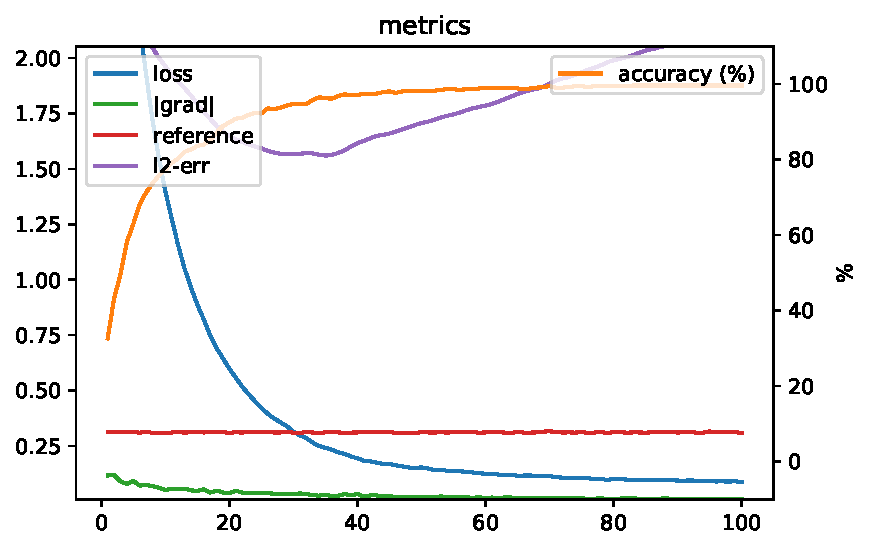
\includegraphics[width=0.7\textwidth]{figures/reconstruction_GMM_NN_ALL_metrics.pdf}
    \caption{Plot of optimization metrics of method NN ALL \\on the GMM data set}
    \label{fig:metrics_GMM_l2_increase}
\end{figure}

\subsubsection{MNIST}


The distortion factor ($\kappa = 0.2$) on the MNIST data set was chosen to be fairly strong.
After distortion, the overall accuracies drop from 97-99\% to near random guesses $\frac 1 C \approx 10\%$
as seen in \cref{tab:mnist_baseline}.
The results for the reconstruction task for all methods on the MNIST data set is depicted in \cref{tab:mnist_results}.
The criterion (CRITERION) alone gives good results on the main network, but fails to generalize when tested on a secondary network.
This shows that the reconstruction is being heavily biased by what the neural network deems to be "correct" images. Although these features might not be robust in the sense that they don't correspond to features we as humans might make out.
The hardly improved verification score of NN, where additionally the second-to-last layer is 
incorporated, seems to confirm
the network's bias in the optimization procedure. 
An improvement in generalization can be seen only after taking 
all layers of the neural network (NN ALL) into account.
The randomly initialized neural network (RANDOM NN) does not add any significant improvement; 
it seems as though it is not able to capture much useful information about the data set.
Random projections (RP) is able to add an additional amount of regularization that is seen in the generalization scores.
Combining the methods (COMBINED) seems to merit overall good scores which can be verified in image quality.


\begin{table}[!htbp]
\centering
\footnotesize
\pgfplotstabletypeset[
results,
images,
display columns/0/.style={column name=\textbf{baseline}, column type=l, string type},
]{figures/reconstruction_MNIST_baseline.csv}
\caption{MNIST baseline scores}
\label{tab:mnist_baseline}
\end{table}

\begin{table}[!htbp]
\centering
\footnotesize
\pgfplotstabletypeset[
results,
images,
every row 11 column 1/.style={highlight},
every row 11 column 2/.style={highlight},
every row 11 column 3/.style={highlight},
every row 11 column 4/.style={highlight},
every row 5 column 5/.style={highlight},
every row 6 column 6/.style={highlight},
]{figures/reconstruction_MNIST_results.csv}
\caption{Metrics on reconstruction results after 100 optimization epochs on MNIST data set}
\label{tab:mnist_results}
\end{table}


Here, it is important to note that the l2-error and the PSNR-score do not improve after the reconstruction task is performed.
Comparing these findings with the qualitative results shown in \cref{AppendixResults}, 
leads to the conclusion that these scores are not actually indicative of image quality.
These scores rely on per-pixel comparisons, and the reconstruction network may introduce shifts in the final image
that can greatly disrupt the score of these metrics.
The SSIM-score seems to be a more robust metric, subjectively seen in image quality.





\subsubsection{CIFAR10}

The CIFAR10 data set is a more complex data set compared to the previous two.
The objects of interest have greatly varying backgrounds and are shown from numerous different angles.
The learned feature representations have to be able to filter out the noise from the signal more than in
the previous data sets.
The network for this data set is of a deeper (34 layers) architecture, and the
the learned feature representations seem to be more robust and correlate more with the verification network.
Comparing the results of the methods that use the representations of the main network (NN, NN ALL)
to the randomly initialized network (RANDOM NN), it can be said that a good feature representation is necessary.
Random projections do not perform well on this task, as their design is too simple to be able to capture complex features.

\begin{table}[!htbp]
\label{tab:cifar10baseline}
\centering
\footnotesize
\pgfplotstabletypeset[
results,
images,
display columns/0/.style={column name=\textbf{Baseline}, column type=l, string type},
]{figures/reconstruction_CIFAR10_baseline.csv}
\caption{CIFAR10 baseline scores}
\end{table}

\begin{table}[!htbp]
\label{tab:cifar10results}
\centering
\footnotesize
\pgfplotstabletypeset[
results,
images,
every row 2 column 1/.style={highlight},
every row 4 column 1/.style={highlight},
every row 3 column 2/.style={highlight},
every row 4 column 3/.style={highlight},
every row 3 column 4/.style={highlight},
every row 3 column 5/.style={highlight},
every row 3 column 6/.style={highlight},
]{figures/reconstruction_CIFAR10_results.csv}
\caption{Metrics on reconstruction results after 100 optimization epochs for CIFAR10}
\end{table}





Of the methods using neural networks, NN ALL has the overall best performance.
This can be confirmed by visual inspection in \cref{AppendixResults}.
By using the class-conditional version (NN ALL CC), one would expect better results.
However, this is not seen in the results and the images appear qualitatively worse. 
A reason why could be that the network is already complex enough to "split" the signal into distinct enough paths so that adding
a class-conditional formulation does not add more context.
It might even be a hindrance, because of the high variance in image statistics
from one image to another due to background "noise".
Since the class-conditional formulation groups inputs according to their respective classes, 
it is possible that, due to random sampling, one iteration contains 
few samples of one class. Alternatively, one grouped batch could
display unusual statistics (e.g. all having red backgrounds), whereas otherwise these would be averaged out.
This in turn can lead to a spike in the loss, resulting in large gradients that affect the optimization.
% NN ALL doesn't suffer from this, as irregularities are smoothed out by larger batches.
\Cref{fig:layer_losses} shows the loss resulting from the difference in the mean
between the source and the target, plotted for each layer.
While the normal formulation is able to minimize statistics over all layers relatively uniformly,
the class-conditional variation struggles with the early layers.
These exhibit higher losses that the reconstruction network is not able to minimize.
Solutions to this problem could entail an increase of the batch size
or, employing another batching method that randomly cycles over all classes
and then selects a batch accordingly. 
This could smooth out irregularities that arise from too few samples.
Alternatively, the losses could be weighted by their layer, giving lower importance to earlier layers. 
Or a hybrid approach could be constructed that only uses class information in later layers.

\begin{figure}
    \centerline{
    \hspace*{6mm}
    \begin{minipage}{0.6\textwidth}
    \caption*{NN ALL}
    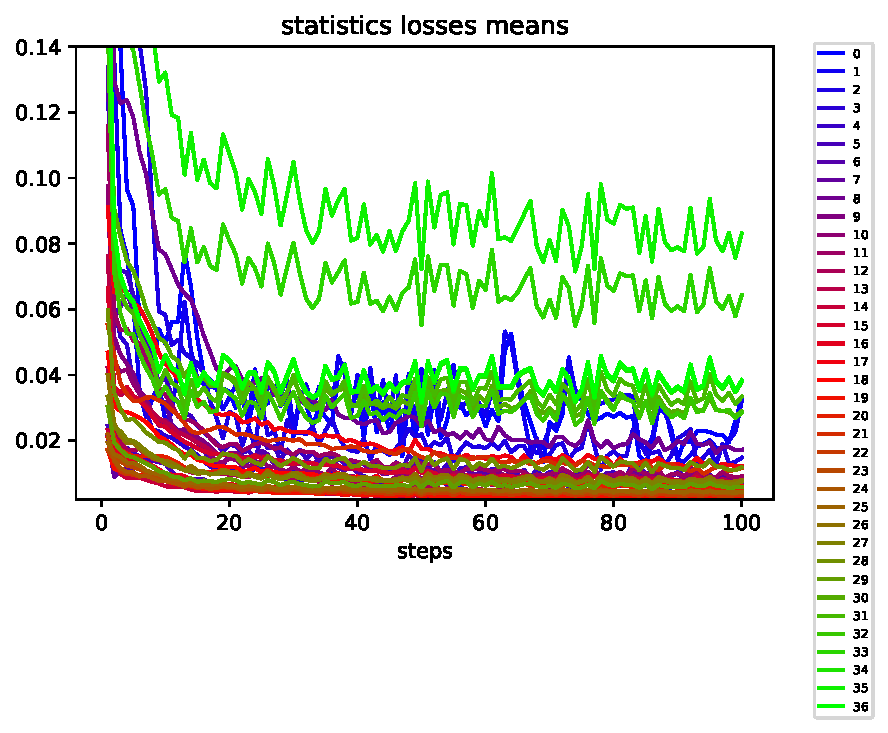
\includegraphics[
    width=\textwidth, 
    trim={0 0 0 0.6cm}, clip,
    ]{figures/reconstruction_CIFAR10_NN_ALL_metrics_statistics_losses_means.pdf}
    \end{minipage}%
    \begin{minipage}{0.6\textwidth}
    \caption*{NN ALL CC}
    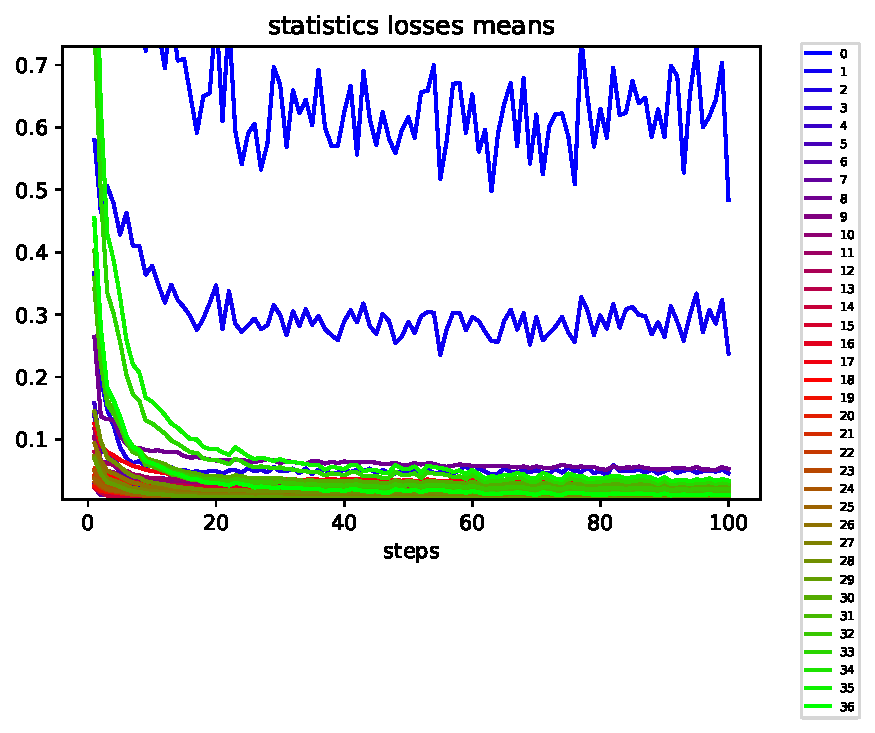
\includegraphics[
    width=\textwidth,
    trim={0 0 0 0.6cm}, clip,
    ]{figures/reconstruction_CIFAR10_NN_ALL_CC_metrics_statistics_losses_means.pdf}
    \end{minipage}
    }
    \caption{Loss coming from the difference in mean batch-statistics plotted per layer. 
    Lighter colors correspond to later layers in the network. \textit{Layer 0} is the input itself.}
    \label{fig:layer_losses}
\end{figure}

\begin{table}[!htbp]
\label{tab:cifar10results_unsupervised}
\centering
\footnotesize
\pgfplotstabletypeset[
results,
images,
% every row 2 column 1/.style={highlight},
% every row 4 column 1/.style={highlight},
% every row 3 column 2/.style={highlight},
% every row 4 column 3/.style={highlight},
% every row 3 column 4/.style={highlight},
% every row 3 column 5/.style={highlight},
% every row 3 column 6/.style={highlight},
]{figures/unsupervised/reconstruction_CIFAR10_results.csv}
\caption{Metrics on reconstruction results after 100 optimization epochs for CIFAR10}
\end{table}


In conclusion, it can be said that 
using the proposed loss formulations NN ALL and NN ALL CC can significantly 
aid in the reconstruction task.
While random projections might be 
able to capture relevant features 
for low-dimensional or comparatively simple data, 
their practical use for complex image data sets is questionable.
Incorporating the non-linearity ReLU in the random projections (RP ReLU), in general, 
does not yield any notable differences in the performances.
This shows that the strength of the neural networks feature-representation
must come from the depth and hierarchical composition of convolutional feature extractors.
The increase in performance compared to a randomly initialized neural network
further shows that learned feature-representations can more efficiently capture
information about the data set.
The final effect of the class-conditional formulation is still to be verified.

\subsection{Qualitative Results on Image Data Sets}

\subsubsection{MNIST}

\begin{figure}[h]
{
    \centering
    \setlength{\abovecaptionskip}{0pt plus 0pt minus 0pt}
    \setlength{\belowcaptionskip}{10pt plus 0pt minus 0pt}
    
    \caption*{\normalsize{\textit{Ground Truth}}}
    \rule{0.4\textwidth}{.4pt}
    
    \centerline{\hspace*{8mm}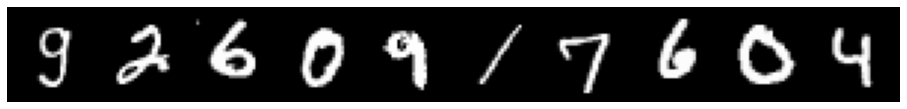
\includegraphics[width=1.4\textwidth]{figures/reconstruction_MNIST_ground_truth.png}}
    \caption*{\normalsize{\textit{Distorted}}}
    \rule{0.4\textwidth}{.4pt}
    
    \centerline{\hspace*{8mm}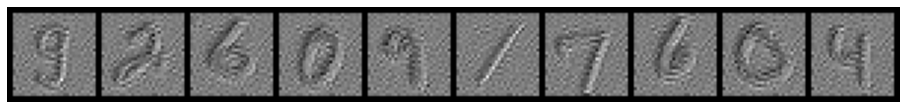
\includegraphics[width=1.4\textwidth]{figures/reconstruction_MNIST_distorted.png}}
    \caption*{\normalsize{CRITERION}}
    \rule{0.4\textwidth}{.4pt}
    
    \centerline{\hspace*{8mm}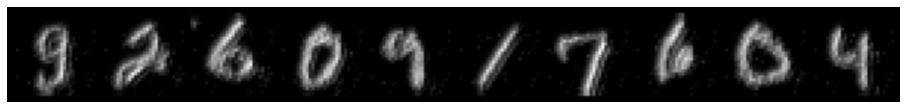
\includegraphics[width=1.4\textwidth]{figures/reconstruction_MNIST_CRITERION_epoch_100.png}}
    \caption*{\normalsize{NN}}
    \rule{0.4\textwidth}{.4pt}
    
    \centerline{\hspace*{8mm}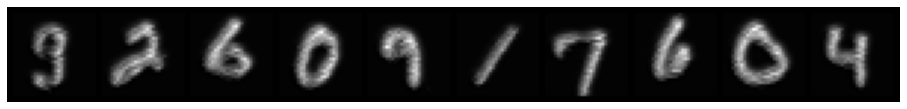
\includegraphics[width=1.4\textwidth]{figures/reconstruction_MNIST_NN_epoch_100.png}}
    \caption*{\normalsize{NN CC}}
    \rule{0.4\textwidth}{.4pt}
    
    \centerline{\hspace*{8mm}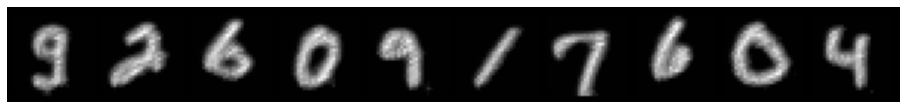
\includegraphics[width=1.4\textwidth]{figures/reconstruction_MNIST_NN_CC_epoch_100.png}}
    \caption*{\normalsize{NN ALL}}
    \rule{0.4\textwidth}{.4pt}
    
    \centerline{\hspace*{8mm}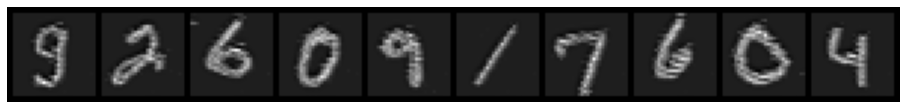
\includegraphics[width=1.4\textwidth]{figures/reconstruction_MNIST_NN_ALL_epoch_100.png}}
    \caption*{\normalsize{NN ALL CC}}
    \rule{0.4\textwidth}{.4pt}
    
    \centerline{\hspace*{8mm}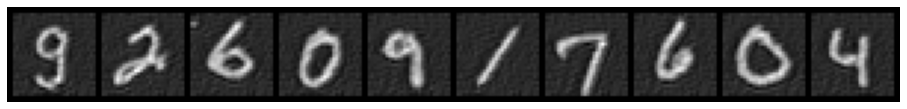
\includegraphics[width=1.4\textwidth]{figures/reconstruction_MNIST_NN_ALL_CC_epoch_100.png}}
}
\end{figure}
\begin{figure}[h]
    \centering
    \setlength{\abovecaptionskip}{0pt plus 0pt minus 0pt}
    \setlength{\belowcaptionskip}{10pt plus 0pt minus 0pt}
    \caption*{\normalsize{RANDOM NN}}
    \rule{0.4\textwidth}{.4pt}
    
    \centerline{\hspace*{8mm}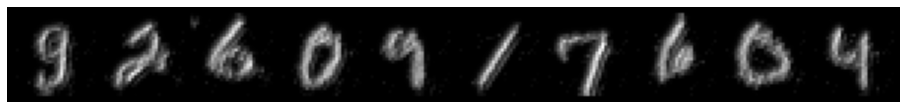
\includegraphics[width=1.4\textwidth]{figures/reconstruction_MNIST_RANDOM_NN_epoch_100.png}}
    \caption*{\normalsize{RANDOM NN CC}}
    \rule{0.4\textwidth}{.4pt}
    
    \centerline{\hspace*{8mm}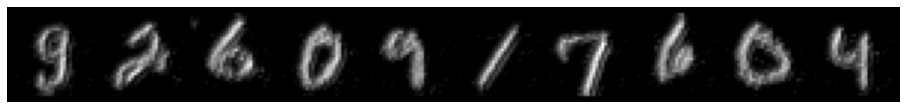
\includegraphics[width=1.4\textwidth]{figures/reconstruction_MNIST_RANDOM_NN_CC_epoch_100.png}}
    \caption*{\normalsize{RP}}
    \rule{0.4\textwidth}{.4pt}
    
    \centerline{\hspace*{8mm}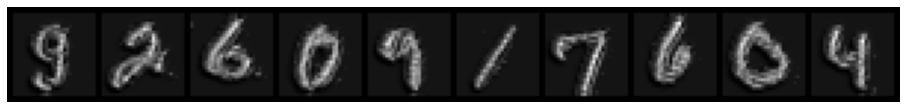
\includegraphics[width=1.4\textwidth]{figures/reconstruction_MNIST_RP_epoch_100.png}}
    \caption*{\normalsize{RP CC}}
    \rule{0.4\textwidth}{.4pt}
    
    \centerline{\hspace*{8mm}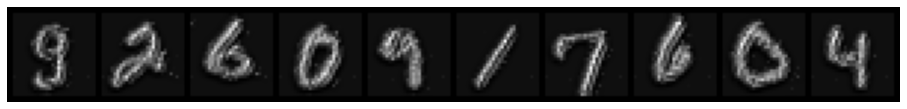
\includegraphics[width=1.4\textwidth]{figures/reconstruction_MNIST_RP_CC_epoch_100.png}}
    \caption*{\normalsize{RP ReLU}}
    \rule{0.4\textwidth}{.4pt}
    
    \centerline{\hspace*{8mm}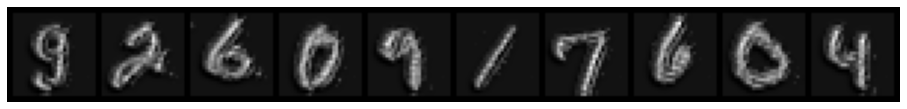
\includegraphics[width=1.4\textwidth]{figures/reconstruction_MNIST_RP_ReLU_epoch_100.png}}
    \caption*{\normalsize{RP ReLU CC}}
    \rule{0.4\textwidth}{.4pt}
    
    \centerline{\hspace*{8mm}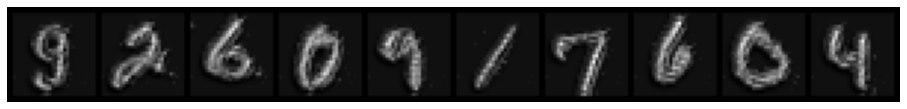
\includegraphics[width=1.4\textwidth]{figures/reconstruction_MNIST_RP_ReLU_CC_epoch_100.png}}
    \caption*{\normalsize{COMBINED CC}}
    \rule{0.4\textwidth}{.4pt}
    
    \centerline{\hspace*{8mm}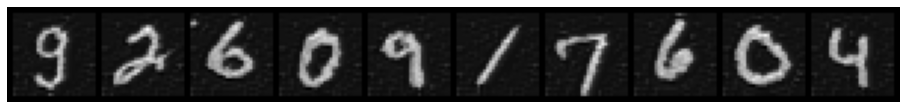
\includegraphics[width=1.4\textwidth]{figures/reconstruction_MNIST_COMBINED_CC_epoch_100.png}}
    
    \caption{Qualitative results of the reconstruction task on MNIST data set after 100 epochs}
    \label{fig:MNIST_Images}
\end{figure}



\subsubsection{CIFAR10}

\begin{figure}[h]
    \centering
    \setlength{\abovecaptionskip}{0pt plus 0pt minus 0pt}
    \setlength{\belowcaptionskip}{10pt plus 0pt minus 0pt}
    \caption*{\normalsize{\textit{Ground Truth}}}
    \rule{0.4\textwidth}{.4pt}
    
    \centerline{\hspace*{8mm}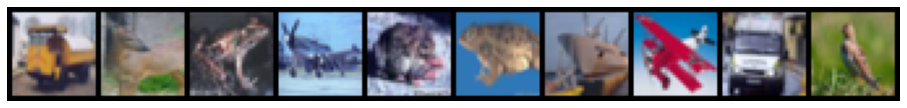
\includegraphics[width=1.4\textwidth]{figures/reconstruction_CIFAR10_ground_truth.png}}
    \caption*{\normalsize{\textit{Distorted}}}
    \rule{0.4\textwidth}{.4pt}
    
    \centerline{\hspace*{8mm}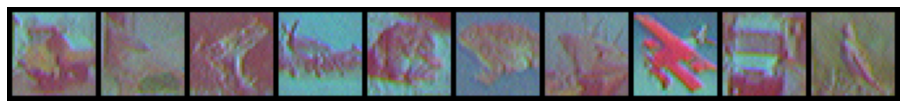
\includegraphics[width=1.4\textwidth]{figures/reconstruction_CIFAR10_distorted.png}}
    \caption*{\normalsize{CRITERION}}
    \rule{0.4\textwidth}{.4pt}
    
    \centerline{\hspace*{8mm}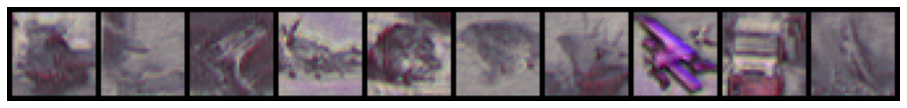
\includegraphics[width=1.4\textwidth]{figures/reconstruction_CIFAR10_CRITERION_epoch_100.png}}
    \caption*{\normalsize{NN}}
    \rule{0.4\textwidth}{.4pt}
    
    \centerline{\hspace*{8mm}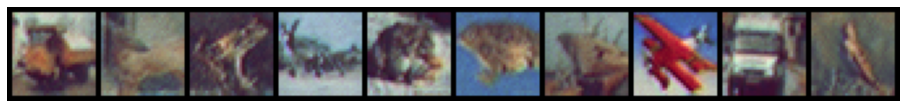
\includegraphics[width=1.4\textwidth]{figures/reconstruction_CIFAR10_NN_epoch_100.png}}
    \caption*{\normalsize{NN CC}}
    \rule{0.4\textwidth}{.4pt}
    
    \centerline{\hspace*{8mm}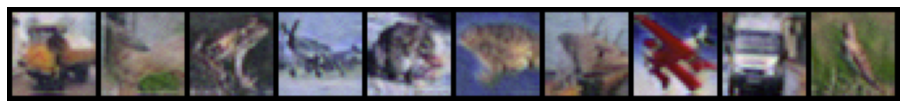
\includegraphics[width=1.4\textwidth]{figures/reconstruction_CIFAR10_NN_CC_epoch_100.png}}
    \caption*{\normalsize{NN ALL}}
    \rule{0.4\textwidth}{.4pt}
    
    \centerline{\hspace*{8mm}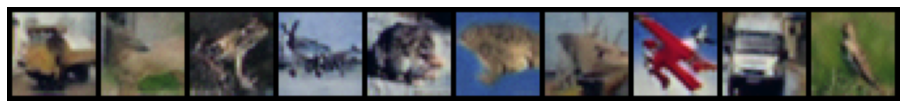
\includegraphics[width=1.4\textwidth]{figures/reconstruction_CIFAR10_NN_ALL_epoch_100.png}}
    \caption*{\normalsize{NN ALL CC}}
    \rule{0.4\textwidth}{.4pt}
    
    \centerline{\hspace*{8mm}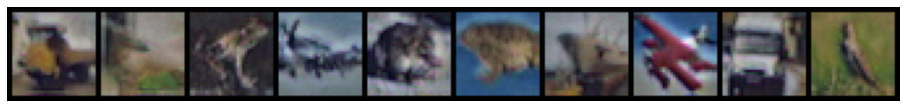
\includegraphics[width=1.4\textwidth]{figures/reconstruction_CIFAR10_NN_ALL_CC_epoch_100.png}}
\end{figure}

\begin{figure}[h]
    \centering
    \setlength{\abovecaptionskip}{0pt plus 0pt minus 0pt}
    \setlength{\belowcaptionskip}{10pt plus 0pt minus 0pt}
    \caption*{\normalsize{RANDOM NN}}
    \rule{0.4\textwidth}{.4pt}
    
    \centerline{\hspace*{8mm}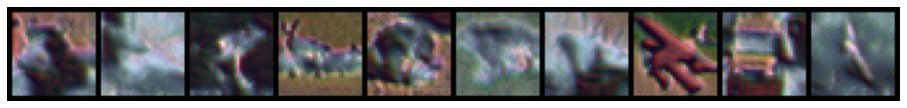
\includegraphics[width=1.4\textwidth]{figures/reconstruction_CIFAR10_RANDOM_NN_epoch_100.png}}
    \caption*{\normalsize{RANDOM NN CC}}
    \rule{0.4\textwidth}{.4pt}
    
    \centerline{\hspace*{8mm}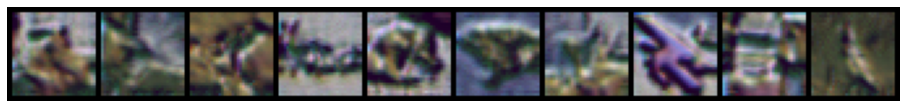
\includegraphics[width=1.4\textwidth]{figures/reconstruction_CIFAR10_RANDOM_NN_CC_epoch_100.png}}
    \caption*{\normalsize{RP}}
    \rule{0.4\textwidth}{.4pt}
    
    \centerline{\hspace*{8mm}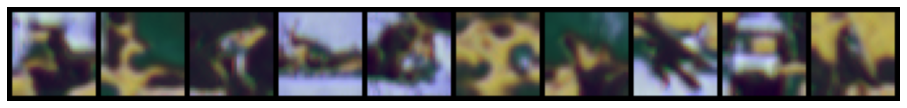
\includegraphics[width=1.4\textwidth]{figures/reconstruction_CIFAR10_RP_epoch_100.png}}
    \caption*{\normalsize{RP CC}}
    \rule{0.4\textwidth}{.4pt}
    
    \centerline{\hspace*{8mm}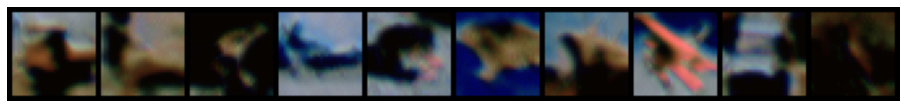
\includegraphics[width=1.4\textwidth]{figures/reconstruction_CIFAR10_RP_CC_epoch_100.png}}
    \caption*{\normalsize{RP ReLU}}
    \rule{0.4\textwidth}{.4pt}
    
    \centerline{\hspace*{8mm}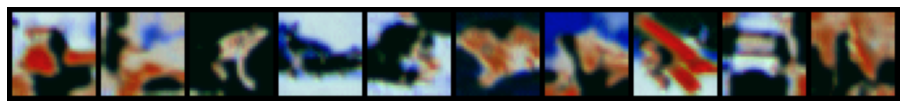
\includegraphics[width=1.4\textwidth]{figures/reconstruction_CIFAR10_RP_ReLU_epoch_100.png}}
    \caption*{\normalsize{RP ReLU CC}}
    \rule{0.4\textwidth}{.4pt}
    
    \centerline{\hspace*{8mm}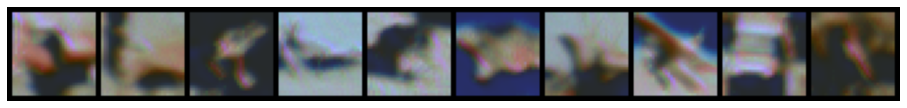
\includegraphics[width=1.4\textwidth]{figures/reconstruction_CIFAR10_RP_ReLU_CC_epoch_100.png}}
    \caption*{\normalsize{COMBINED CC}}
    \rule{0.4\textwidth}{.4pt}
    
    \centerline{\hspace*{8mm}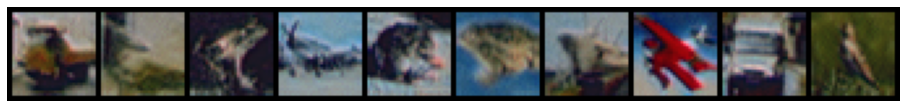
\includegraphics[width=1.4\textwidth]{figures/reconstruction_CIFAR10_COMBINED_CC_epoch_100.png}}
    
    \caption{Qualitative results of the reconstruction task on CIFAR10 data set after 100 epochs}
    \label{fig:CIFAR_Images}
\end{figure}



\begin{figure}[h]
    \centering
    \setlength{\abovecaptionskip}{0pt plus 0pt minus 0pt}
    \setlength{\belowcaptionskip}{10pt plus 0pt minus 0pt}
    \caption*{\normalsize{\textit{Ground Truth}}}
    \rule{0.4\textwidth}{.4pt}
    
    \centerline{\hspace*{8mm}
\includegraphics[width=1.4\textwidth]{figures/unsupervised/reconstruction_CIFAR10_ground_truth.png}}
    \caption*{\normalsize{\textit{Distorted}}}
    \rule{0.4\textwidth}{.4pt}
    
    \centerline{\hspace*{8mm}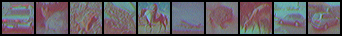
\includegraphics[width=1.4\textwidth]{figures/unsupervised/reconstruction_CIFAR10_distorted.png}}
    
    \caption*{\normalsize{NN}}
    \rule{0.4\textwidth}{.4pt}
    
    \centerline{\hspace*{8mm}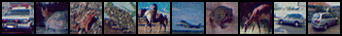
\includegraphics[width=1.4\textwidth]{figures/unsupervised/reconstruction_CIFAR10_NN_epoch_100.png}}
    \caption*{\normalsize{NN ALL}}
    \rule{0.4\textwidth}{.4pt}
    
    \centerline{\hspace*{8mm}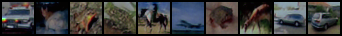
\includegraphics[width=1.4\textwidth]{figures/unsupervised/reconstruction_CIFAR10_NN_ALL_epoch_100.png}}
    
    \caption*{\normalsize{RANDOM NN}}
    \rule{0.4\textwidth}{.4pt}
    
    \centerline{\hspace*{8mm}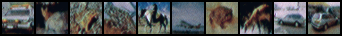
\includegraphics[width=1.4\textwidth]{figures/unsupervised/reconstruction_CIFAR10_RANDOM_NN_epoch_100.png}}
    \caption*{\normalsize{RP}}
    \rule{0.4\textwidth}{.4pt}
    
    \centerline{\hspace*{8mm}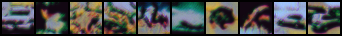
\includegraphics[width=1.4\textwidth]{figures/unsupervised/reconstruction_CIFAR10_RP_epoch_100.png}}
    
    \caption{Qualitative results of the reconstruction task on CIFAR10 data set in an unsupervised setting after 100 epochs}

    \label{fig:CIFAR_Images_unsupervised}
\end{figure}

\begin{figure}[h]
    \centering
    \setlength{\abovecaptionskip}{0pt plus 0pt minus 0pt}
    \setlength{\belowcaptionskip}{10pt plus 0pt minus 0pt}
\end{figure}





\begin{figure}[h]
    \centering
    \setlength{\abovecaptionskip}{0pt plus 0pt minus 0pt}
    \setlength{\belowcaptionskip}{10pt plus 0pt minus 0pt}
    
    \caption*{\normalsize{CRITERION}}
    \rule{0.4\textwidth}{.4pt}
    
    \centerline{\hspace*{8mm}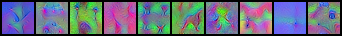
\includegraphics[width=1.4\textwidth]{figures/inversion_CIFAR10_CRITERION_epoch_3000.png}}
    \caption*{\normalsize{NN}}
    \rule{0.4\textwidth}{.4pt}
    
    \centerline{\hspace*{8mm}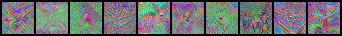
\includegraphics[width=1.4\textwidth]{figures/inversion_CIFAR10_NN_epoch_3000.png}}
    \caption*{\normalsize{NN CC}}
    \rule{0.4\textwidth}{.4pt}
    
    \centerline{\hspace*{8mm}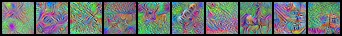
\includegraphics[width=1.4\textwidth]{figures/inversion_CIFAR10_NN_CC_epoch_3000.png}}
    \caption*{\normalsize{NN ALL}}
    \rule{0.4\textwidth}{.4pt}
    
    \centerline{\hspace*{8mm}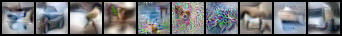
\includegraphics[width=1.4\textwidth]{figures/inversion_CIFAR10_NN_ALL_epoch_3000.png}}
    \caption*{\normalsize{NN ALL CC}}
    \rule{0.4\textwidth}{.4pt}
    
    \centerline{\hspace*{8mm}
\includegraphics[width=1.4\textwidth]{figures/inversion_CIFAR10_NN_ALL_CC_epoch_3000.png}}
\end{figure}

\begin{figure}[h]
    \centering
    \setlength{\abovecaptionskip}{0pt plus 0pt minus 0pt}
    \setlength{\belowcaptionskip}{10pt plus 0pt minus 0pt}
    \caption*{\normalsize{RANDOM NN}}
    \rule{0.4\textwidth}{.4pt}
    
    \centerline{\hspace*{8mm}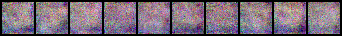
\includegraphics[width=1.4\textwidth]{figures/inversion_CIFAR10_RANDOM_NN_epoch_3000.png}}
    \caption*{\normalsize{RANDOM NN CC}}
    \rule{0.4\textwidth}{.4pt}
    
    \centerline{\hspace*{8mm}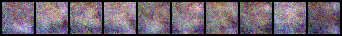
\includegraphics[width=1.4\textwidth]{figures/inversion_CIFAR10_RANDOM_NN_CC_epoch_3000.png}}
    \caption*{\normalsize{RP}}
    \rule{0.4\textwidth}{.4pt}
    
    \centerline{\hspace*{8mm}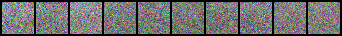
\includegraphics[width=1.4\textwidth]{figures/inversion_CIFAR10_RP_epoch_3000.png}}
    \caption*{\normalsize{RP CC}}
    \rule{0.4\textwidth}{.4pt}
    
    \centerline{\hspace*{8mm}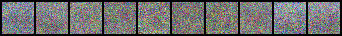
\includegraphics[width=1.4\textwidth]{figures/inversion_CIFAR10_RP_CC_epoch_3000.png}}
    \caption*{\normalsize{RP ReLU}}
    \rule{0.4\textwidth}{.4pt}
    
    \centerline{\hspace*{8mm}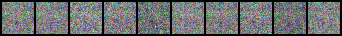
\includegraphics[width=1.4\textwidth]{figures/inversion_CIFAR10_RP_ReLU_epoch_3000.png}}
    \caption*{\normalsize{RP ReLU CC}}
    \rule{0.4\textwidth}{.4pt}
    
    \centerline{\hspace*{8mm}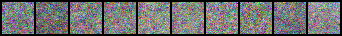
\includegraphics[width=1.4\textwidth]{figures/inversion_CIFAR10_RP_ReLU_CC_epoch_3000.png}}
    \caption*{\normalsize{COMBINED CC}}
    \rule{0.4\textwidth}{.4pt}
    
    \centerline{\hspace*{8mm}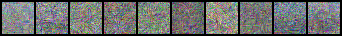
\includegraphics[width=1.4\textwidth]{figures/inversion_CIFAR10_COMBINED_CC_epoch_3000.png}}
    
    \caption{Qualitative results of the inversion task on CIFAR10 data set after 3000 epochs}
    \label{fig:CIFAR_Images}
\end{figure}





\subsection{Hyperparameter-Influence}


In the following, the influence of various hyperparameter settings on the reconstruction outcome is studied.
A grid search is performed on:
\begin{flalign*}
    s_\text{width} &\in \{4, 8, 16\} &\\
    s_\text{depth} &\in \{4, 8, 16\} \\
    n_{\set B} &\in \{128, 512, 1024, 2048\} \\
\end{flalign*}

Every run depicts a hyperparameter setting ($s_\text{width}, s_\text{depth},  n_{\set B}$) of the Cartesian product
of all possible values shown above.

The results for the reconstruction task are plotted in \cref{fig:rec_hyperparameter_search}.

The influence of $n_{\set B}$ on the outcome is quite clear, but the width and the depth of the reconstruction
network is not. In fact, it might even seem as though an increase in complexity of the model is rather
detrimental to the scores.

The findings are solidified in \cref{fig:rec_hyperparameter_heatmap}, where a correlation heat map is given
between the parameters and the scores is given.

While $n_{\set B}$ is clearly positively correlated for all scores 
(except for the l2-error, where a lower score is better), 
the other parameters show an almost inverse effect on what one would expect.
The larger reconstruction models would likely achieve higher scores after a longer training time.






\begin{figure}[!htbp]
\centering
    
    \caption*{\hspace*{6mm}NN ALL CC}
    \centerline{
    \hspace*{6mm}
    \begin{minipage}{0.6\textwidth}
    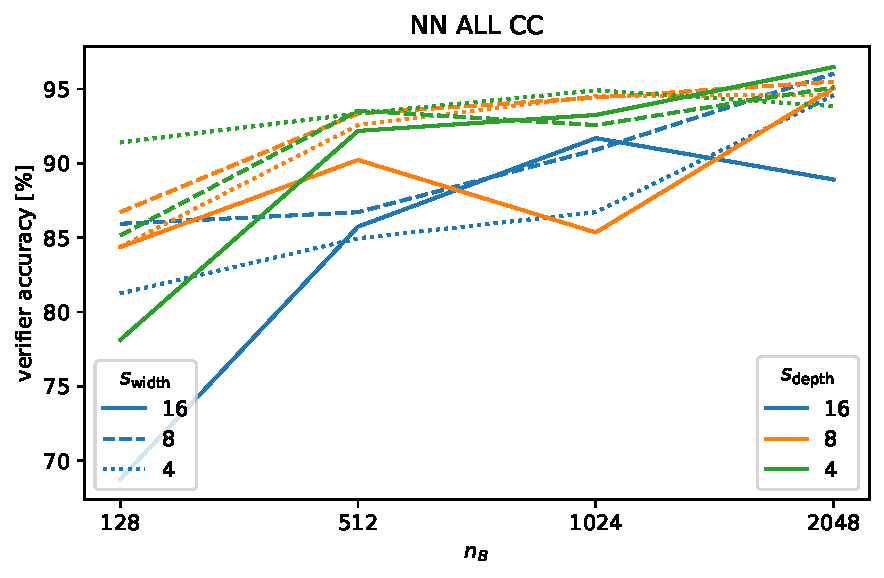
\includegraphics[
    trim={0 0 0 0.6cm}, clip,
    width=\textwidth
    ]{figures/comparison_CIFAR10_hyperparameters_verifier_accuracy_NN_ALL_CC.pdf}
    \end{minipage}%
    \begin{minipage}{0.6\textwidth}
    \includegraphics[
    trim={0 0 0 0.6cm}, clip,
    width=\textwidth
    ]{figures/comparison_CIFAR10_hyperparameters_validation_accuracy_NN_ALL_CC.pdf}
    \end{minipage}
    }
\caption{Reconstruction results for multiple hyperparameter settings on CIFAR10. 
Every data point depicts the end-results after 100 epochs.}
\label{fig:rec_hyperparameter_search}
\end{figure}


\begin{figure}[!htbp]
\centering
\caption*{NN ALL CC}
\includegraphics[
trim={0 0 0 0.75cm}, clip,
width=0.7\textwidth
]{figures/comparison_CIFAR10_hyperparameters_heatmap_NN_ALL_CC.pdf}
\caption{Hyperparameter correlation table}
\label{fig:rec_hyperparameter_heatmap}
\end{figure}




















